\documentclass[border=2pt]{standalone}

\usepackage{tikz}


\begin{document}
\begin{tikzpicture}[]

%\draw[help lines, color=gray!30, dashed] (0,0) grid (20,12);

\node[] at (0,1) (I1) {(a)};
\node[] at (7.5,3.75) (I2) {(b)};
\node[] at (7.5,0) (I3) {(c)};

\node[yshift=110,xshift=-10] at (I1) () {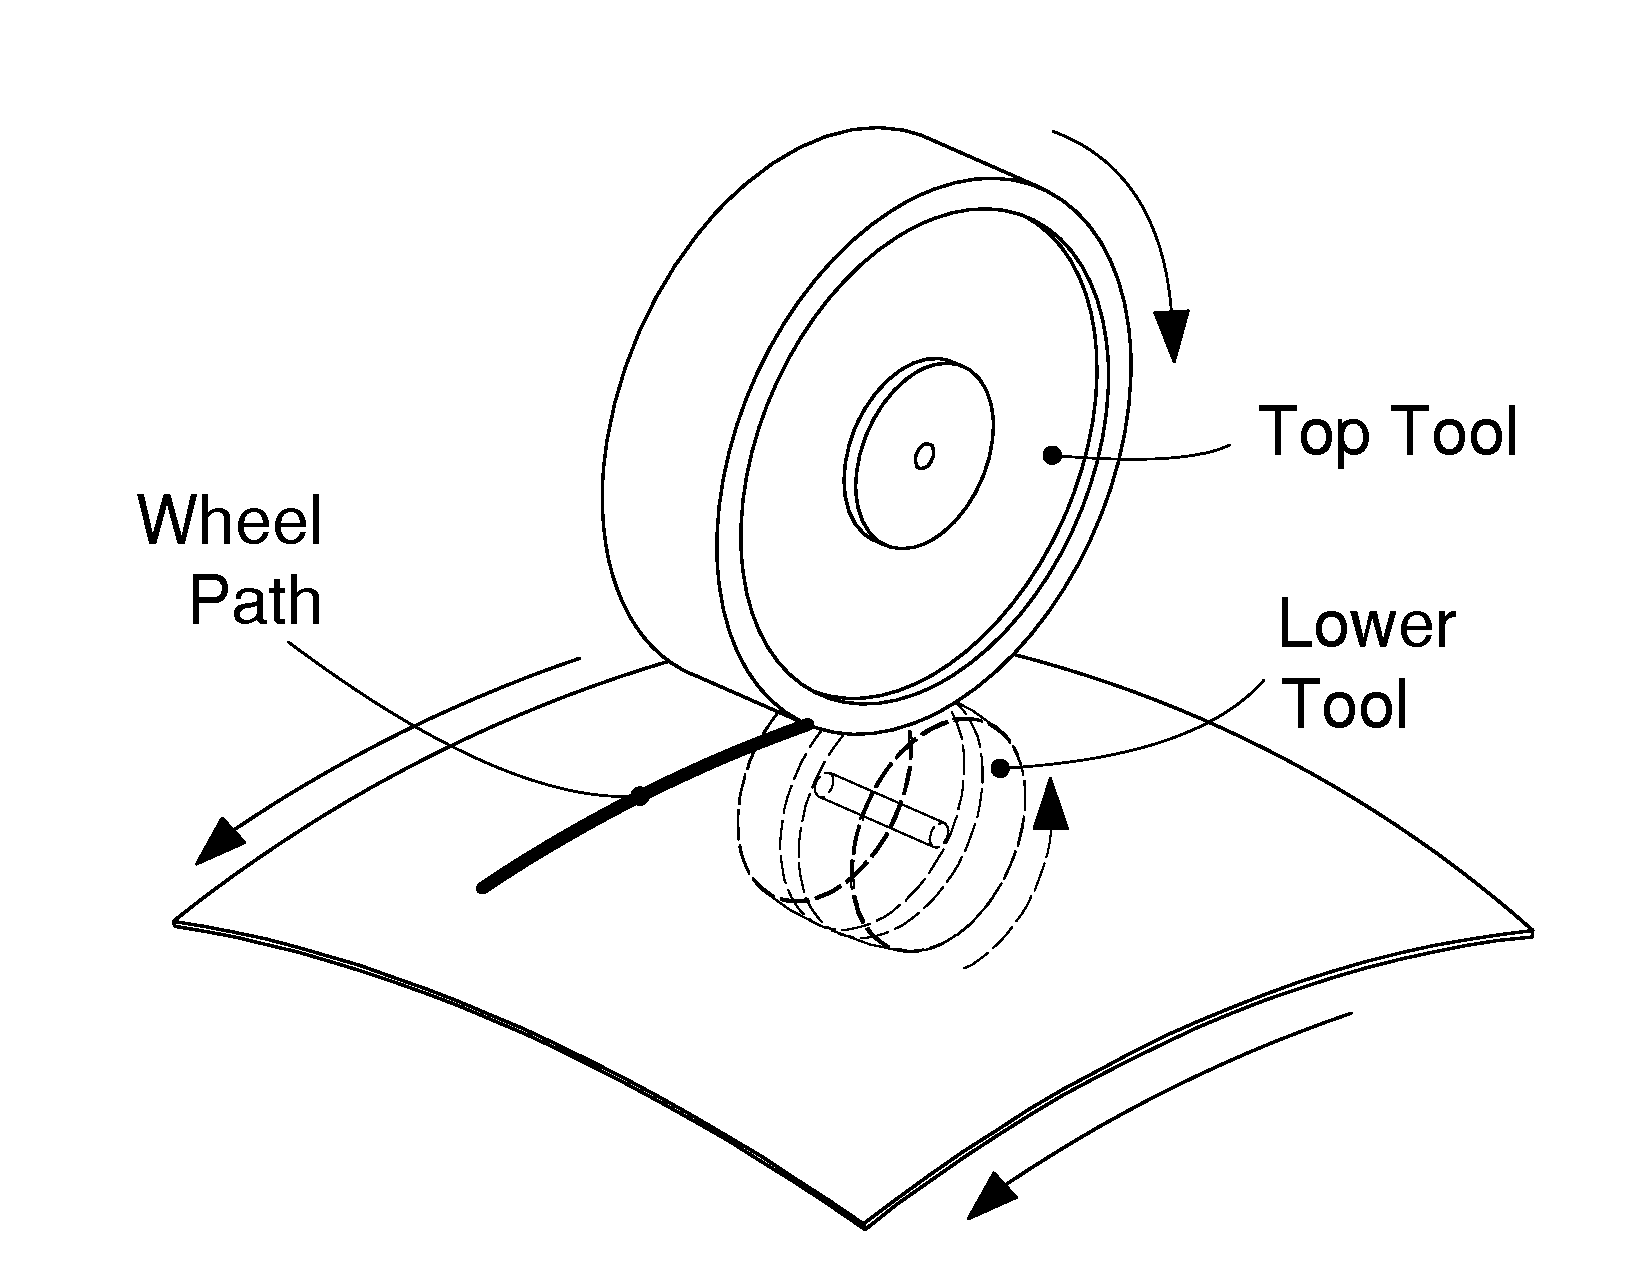
\includegraphics[width=25em]{Images/WheelingTechDrawing1.pdf}};

\node[yshift=90,xshift=-25] at (I2) () {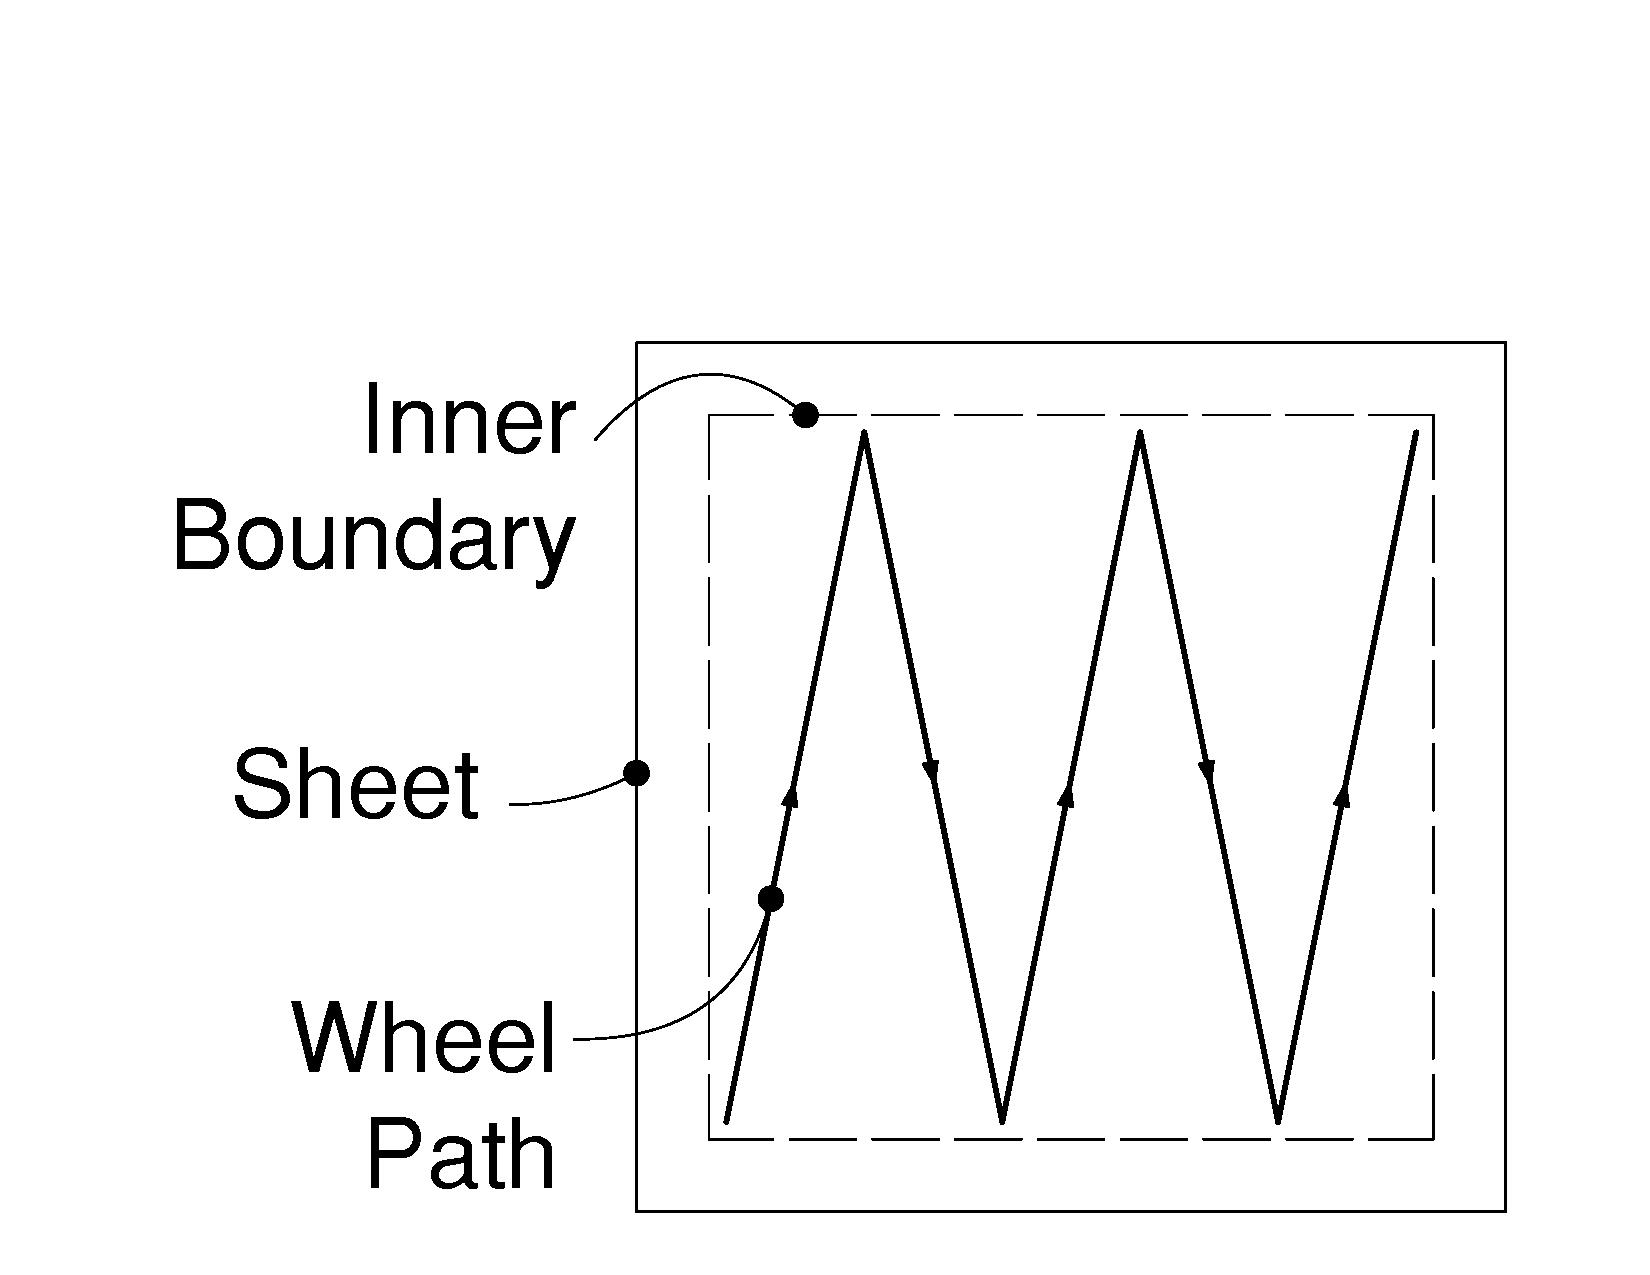
\includegraphics[width=20em]{Images/WheelingTechDrawing2.pdf}};

\node[yshift=80,xshift=-5] at (I3) () {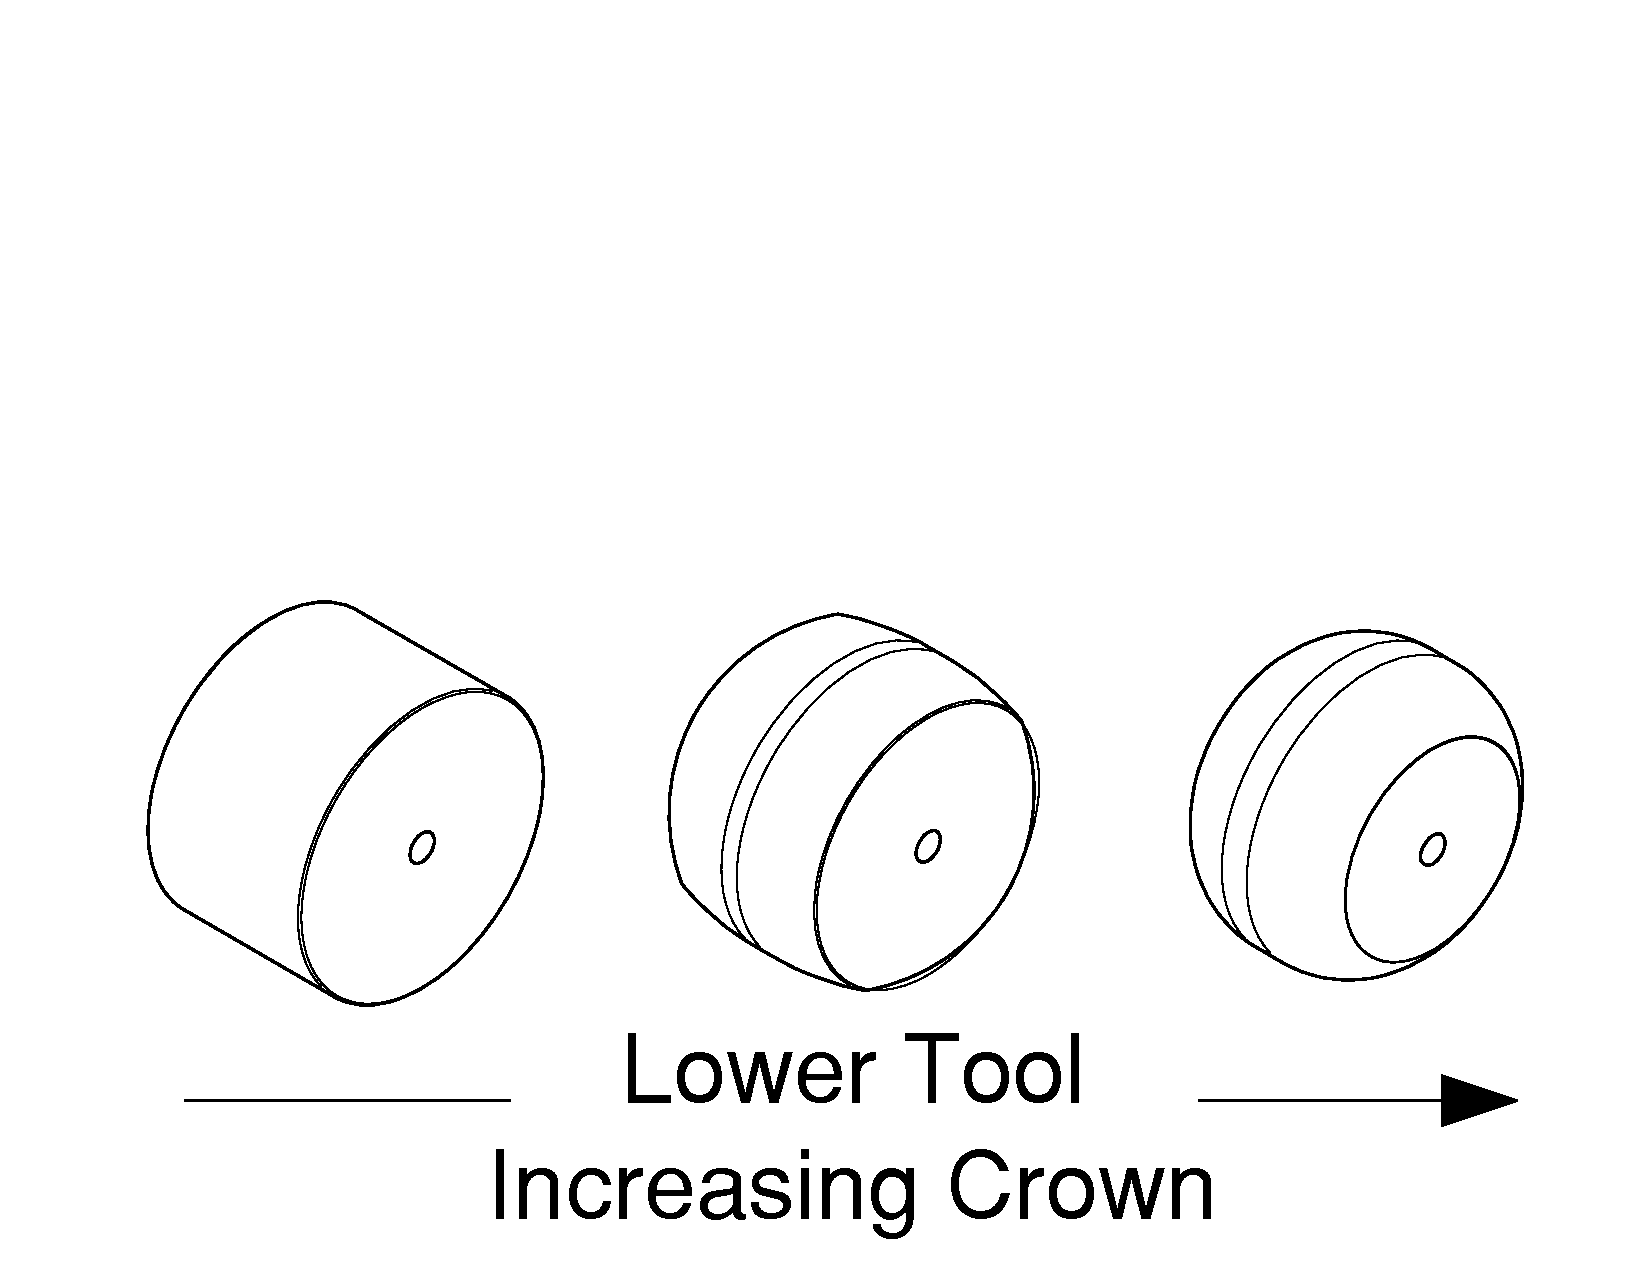
\includegraphics[width=18em]{Images/WheelingTechDrawing3.pdf}};

\end{tikzpicture}
\end{document}